\subsection{Das Interface/Die App}
\label{ssec:interface}

Die App bietet eine Benutzeroberfläche mit verschiedenen Bildschirmen:
\begin{figure}[h]
	\centering
	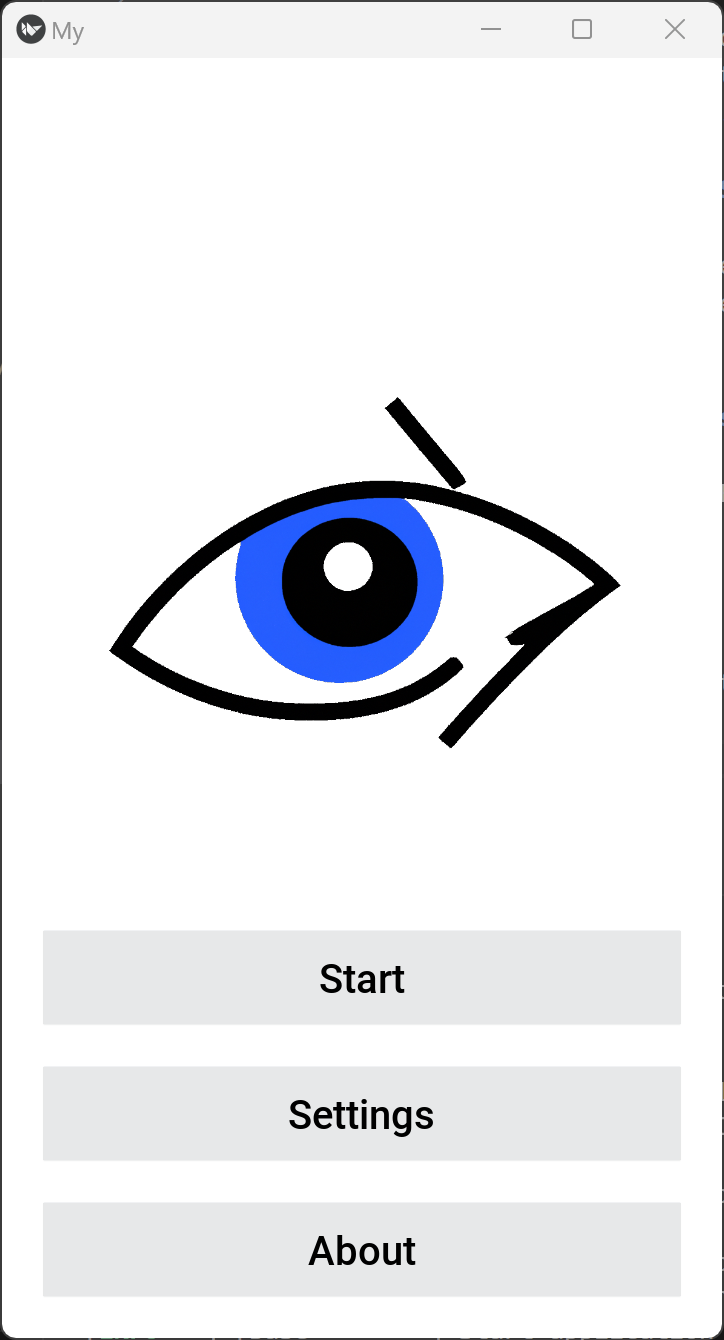
\includegraphics[width=5cm]{images/mainscreen.png} % Ersetzen Sie 'path_to_the_logo.jpg' durch den Pfad zum Logo
	\caption{Hauptbildschirm (MainScreen)}
	\label{fig:mainscreen}
\end{figure}
In \ref{fig:mainscreen} ist der Einstiegsbildschirm der App zu sehen. Hier erhalten Benutzer eine kurze Einführung in die App und können die Müdigkeitserkennung starten oder auf die Einstellungen zugreifen.
\begin{figure}[h]
	\centering
	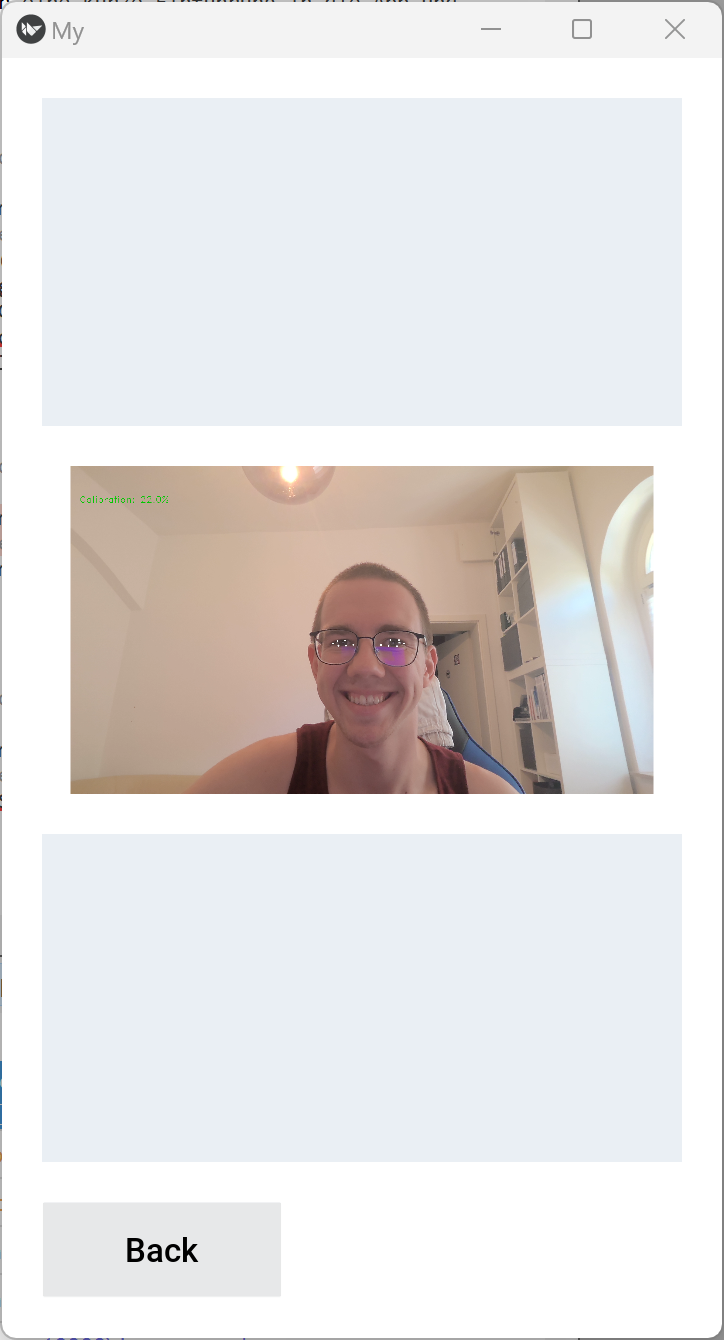
\includegraphics[width=5cm]{images/detectionscreen.png} % Ersetzen Sie 'path_to_the_logo.jpg' durch den Pfad zum Logo
	\caption{Erkennungsbildschirm (DetectionScreen)}
	\label{fig:detectionscreen}
\end{figure}
In \ref{fig:detectionscreen} findet die eigentliche Müdigkeitserkennung statt. Die Kamera zeigt eine Echtzeitansicht, und erkannte Gesichtsmerkmale wie die Augen werden markiert. Bei Erkennung von Müdigkeitsmerkmalen kann die App Warnungen anzeigen oder Alarmtöne abspielen.
\begin{figure}[h]
	\centering
	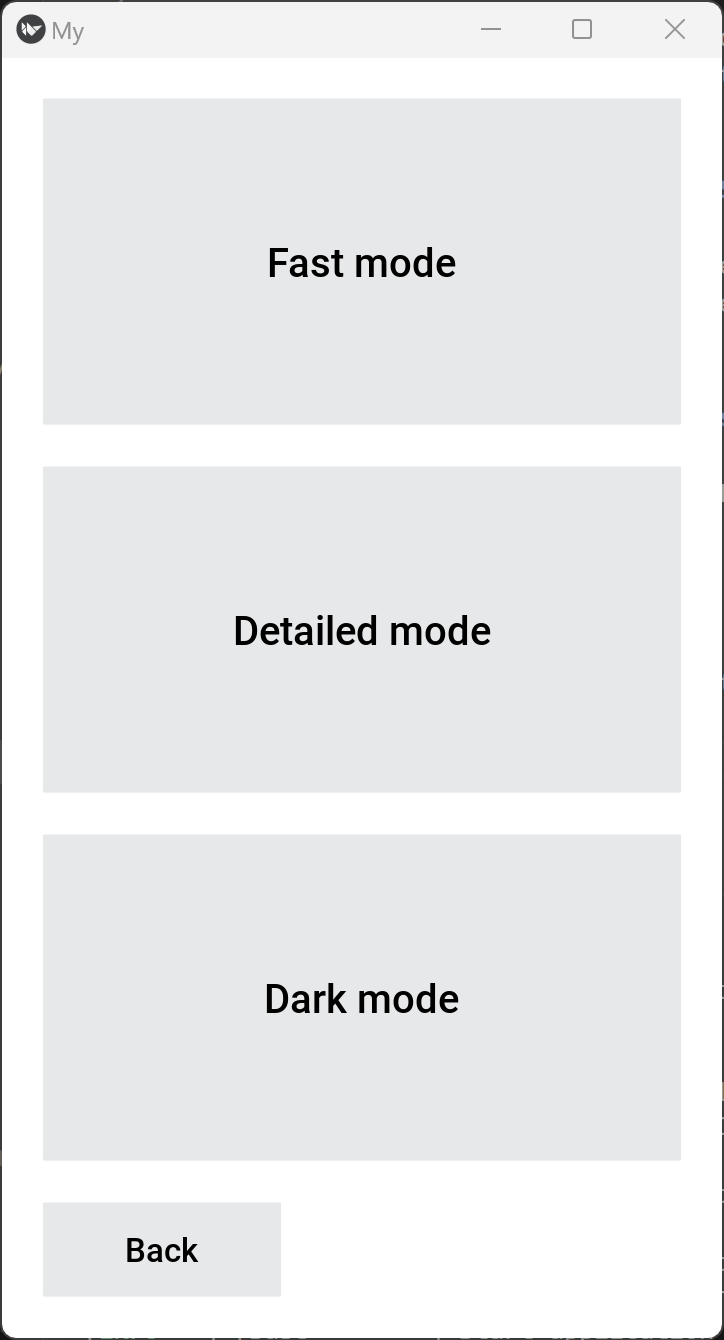
\includegraphics[width=5cm]{images/settingscreen.png} % Ersetzen Sie 'path_to_the_logo.jpg' durch den Pfad zum Logo
	\caption{Einstellungsbildschirm (SettingsScreen)}
	\label{fig:settingscreen}
\end{figure}
In \ref{fig:settingscreen} ist der Einstellungsscreen zu sehen. Benutzer können hier verschiedene Einstellungen für die Benutzeröberfläche anpassen.
\begin{figure}[h]
	\centering
	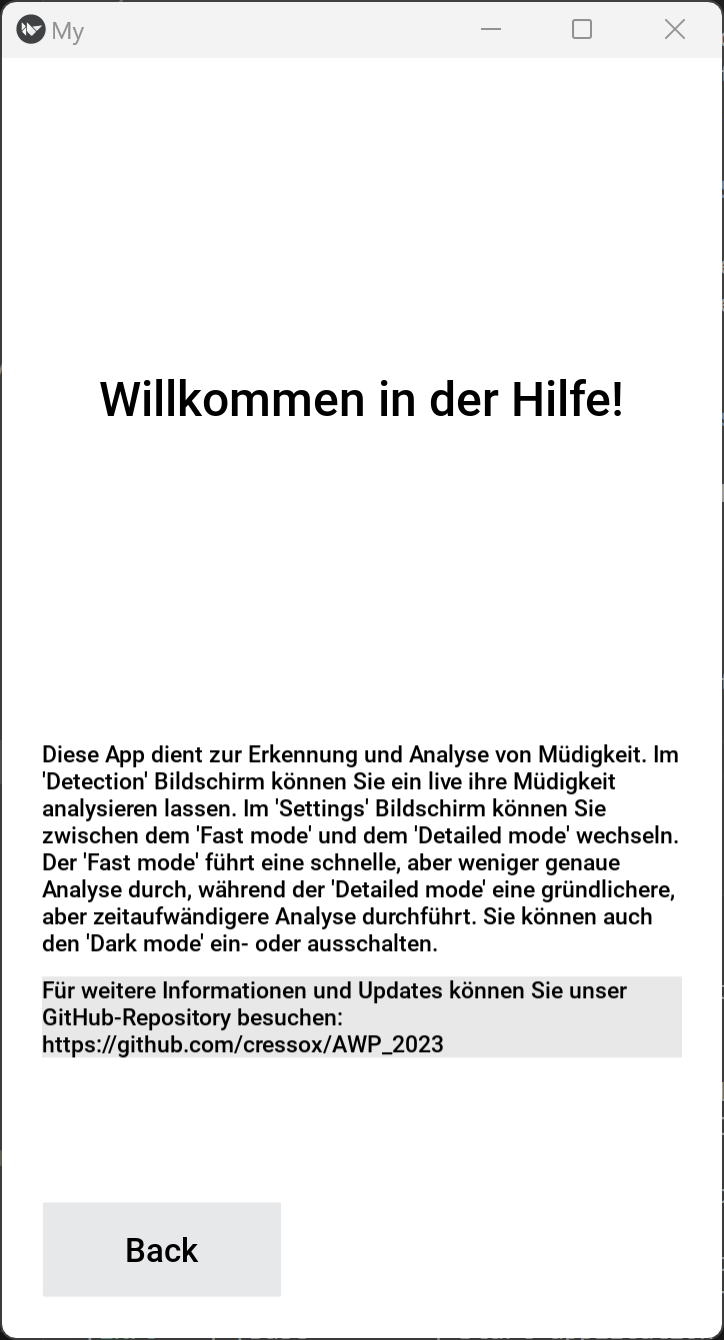
\includegraphics[width=5cm]{images/helpscreen.png} % Ersetzen Sie 'path_to_the_logo.jpg' durch den Pfad zum Logo
	\caption{Hilfebildschirm (HelpScreen)}
	\label{fig:helpscreen}
\end{figure}
In \ref{fig:helpscreen} ist der Hilfebildschirm zu sehen. Dieser Bildschirm bietet detaillierte Informationen zur Verwendung der App und ihrer Funktionen.